\section{Planes and Surfaces}

\subsection{Determining a Plane}

A plane $\mathcal{P}$ in $\mathbb{R}^3$ can be uniquely determined by any of the following geometric data:
\begin{itemize}
    \item A point $Q$ on the plane and a normal vector $\vv{n} \perp \mathcal{P}$.
    \item Three non-collinear points.
    \item A general linear equation $ax + by + cz + d = 0$.
    \item Two intersecting lines (or two non-parallel direction vectors).
    \item Two parallel distinct lines.
    \item A line $\mathcal{L}$ and a point $Q \notin \mathcal{L}$.
\end{itemize}

\subsection{Mathematical Formulations of a Plane}

\textbf{Case 1: Plane passing through the origin $O(0,0,0)$}

A vector $\vv{v} = \ang{x, y, z}$ lies in $\mathcal{P} \iff \vv{v} \perp \vv{n}$, where $\vv{n} = \ang{a, b, c}$:
\[
\vv{v} \in \mathcal{P} \iff \vv{v} \cdot \vv{n} = 0 \iff ax + by + cz = 0
\]
In set notation:
\[
\mathcal{P} = \{ \ang{x, y, z} \mid ax + by + cz = 0 \}
\]

\vspace{0.5em}
\noindent
\begin{minipage}[c]{0.52\textwidth}
\textbf{Case 2: Plane passing through a point $Q(x_0, y_0, z_0)$}

Let $Q$ be a known point on $\mathcal{P}$ with position vector $\vv{OQ} = \ang{x_0, y_0, z_0}$. Any point $W(x, y, z)$ on the plane satisfies:
\[
(\vv{OW} - \vv{OQ}) \perp \vv{n} \iff (\vv{OW} - \vv{OQ}) \cdot \vv{n} = 0
\]
Expanding this dot product yields the point-normal form:
\[
a(x - x_0) + b(y - y_0) + c(z - z_0) = 0
\]
or equivalently:
\[
ax + by + cz = ax_0 + by_0 + cz_0
\]
\end{minipage}%
\hfill
\begin{minipage}[c]{0.44\textwidth}
\centering
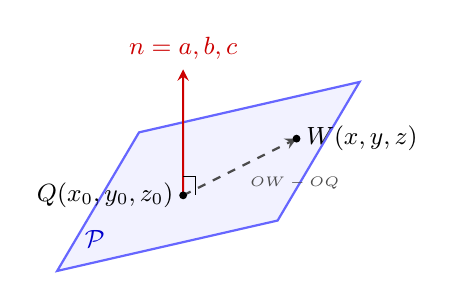
\begin{tikzpicture}[scale=0.8, >=stealth]
    % Draw plane
    \draw[thick, fill=blue!5, draw=blue!60] (0,0) -- (3.5,0.8) -- (4.8,3) -- (1.3,2.2) -- cycle;
    
    % Points
    \coordinate (Q) at (2,1.2);
    \coordinate (W) at (3.8,2.1);
    
    % Vectors
    \draw[->, thick, red!80!black] (Q) -- (2,3.2) node[above] {\small $\vv{n} = \ang{a,b,c}$};
    \draw[->, thick, dashed, black!70] (Q) -- (W) node[midway, below right] {\tiny $\vv{OW}-\vv{OQ}$};
    
    % Right angle sign
    \draw (2,1.5) -- (2.2,1.5) -- (2.2,1.2);
    
    % Point nodes
    \filldraw[black] (Q) circle (1.5pt) node[left] {\small $Q(x_0,y_0,z_0)$};
    \filldraw[black] (W) circle (1.5pt) node[right] {\small $W(x,y,z)$};
    \node[blue!80!black] at (0.6,0.5) {\small $\mathcal{P}$};
\end{tikzpicture}
\end{minipage}

\vspace{0.5em}

We can always scale the coefficients $a, b, c, d$ in $ax + by + cz = d$ by $\frac{1}{\|\vv{n}\|}$ to obtain a unit normal vector $\vv{\hat{n}} = \frac{\ang{a, b, c}}{\sqrt{a^2 + b^2 + c^2}}$.

\subsection{Properties of Normal Vectors}

For any set of vectors $\{\vv{u}, \vv{v}, \vv{w}\}$ where $\vv{v} \nparallel \vv{w}$, the following statements are equivalent:
\begin{itemize}
    \item $\vv{u} \perp \vv{v}$ and $\vv{u} \perp \vv{w}$.
    \item $\vv{u} \parallel (\vv{v} \times \vv{w})$.
    \item $\vv{u} \perp \mathcal{P}$, where $\mathcal{P} = \text{Span}\{\vv{v}, \vv{w}\}$.
\end{itemize}

\begin{problem}{Finding Normal Vectors}{finding_normal_vectors}
Find a normal vector $\vv{n}$ to the plane $\mathcal{P}$ given by the equation $(x - 1) - (y - 1) = 0$.
\end{problem}

\begin{sol}
The equation simplifies to $x - y = 0$. We can extract or compute the normal vector in two ways:

\textbf{Method 1 (Direct Inspection):}
From the general form $ax + by + cz = d$, the coefficients of $x, y, z$ directly give the normal vector:
\[
\vv{n} = \ang{1, -1, 0}
\]

\textbf{Method 2 (Cross Product of Parallel Plane Vectors):}
Two vectors parallel to the plane $\mathcal{P}$ are $\vv{v_1} = \ang{0, 0, 1}$ and $\vv{v_2} = \ang{1, 1, 0}$. Taking their cross product gives:
\[
\vv{n} = \vv{v_1} \times \vv{v_2} = 
\left| \begin{array}{ccc}
\vv{i} & \vv{j} & \vv{k} \\
0 & 0 & 1 \\
1 & 1 & 0
\end{array} \right|
= \vv{i}(0 - 1) - \vv{j}(0 - 1) + \vv{k}(0 - 0) = \ang{-1, 1, 0}
\]
Note that $\ang{-1, 1, 0} = -\ang{1, -1, 0}$, which represents the same normal line direction.
\end{sol}

\begin{problem}{Finding a Plane From Three Points}{find_a_plane}
Find the equation of the plane containing the points $P(1, 0, 1)$, $Q(0, 2, 0)$, and $R(2, 1, 0)$.
\end{problem}

\begin{sol}
\noindent
\begin{minipage}[c]{0.55\textwidth}
\textbf{Step 1: Construct two displacement vectors in the plane}
\begin{align*}
\vv{PQ} &= \ang{0-1, 2-0, 0-1} = \ang{-1, 2, -1} \\
\vv{PR} &= \ang{2-1, 1-0, 0-1} = \ang{1, 1, -1}
\end{align*}

\textbf{Step 2: Compute the normal vector via cross product}
\[
\vv{n} = \vv{PQ} \times \vv{PR} = 
\left| \begin{array}{ccc}
\vv{i} & \vv{j} & \vv{k} \\
-1 & 2 & -1 \\
1 & 1 & -1
\end{array} \right|
= \ang{-1, -2, -3}
\]

\textbf{Step 3: Write the plane equation using point $P(1,0,1)$}
\[
-1(x - 1) - 2(y - 0) - 3(z - 1) = 0 
\]
Simplifying yields:
\[
x + 2y + 3z = 4
\]
\end{minipage}%
\hfill
\begin{minipage}[c]{0.41\textwidth}
\centering
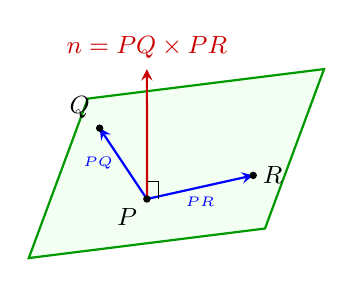
\begin{tikzpicture}[scale=0.75, >=stealth]
    % Plane
    \draw[thick, fill=green!5, draw=green!60!black] (0,0) -- (4,0.5) -- (5,3.2) -- (1,2.7) -- cycle;
    
    % Points
    \coordinate (P) at (2,1);
    \coordinate (Q) at (1.2,2.2);
    \coordinate (R) at (3.8,1.4);
    
    % Vectors in plane
    \draw[->, thick, blue] (P) -- (Q) node[midway, left] {\tiny $\vv{PQ}$};
    \draw[->, thick, blue] (P) -- (R) node[midway, below] {\tiny $\vv{PR}$};
    
    % Normal vector
    \draw[->, thick, red!80!black] (P) -- (2,3.2) node[above] {\small $\vv{n} = \vv{PQ} \times \vv{PR}$};
    
    % Right angle symbol
    \draw (2,1.3) -- (2.2,1.3) -- (2.2,1);
    
    % Point marks
    \filldraw[black] (P) circle (1.5pt) node[below left] {\small $P$};
    \filldraw[black] (Q) circle (1.5pt) node[above left] {\small $Q$};
    \filldraw[black] (R) circle (1.5pt) node[right] {\small $R$};
\end{tikzpicture}
\end{minipage}
\end{sol}


\section{Spheres and Planes}

\subsection{Determining a Sphere}
A sphere in $\mathbb{R}^3$ can be uniquely determined by any of the following sets of data:
\begin{itemize}
    \item A center point $(a,b,c) \in \mathbb{R}^3$ and a radius $R \in \mathbb{R}^{>0}$.
    \item Two points representing the endpoints of a diameter.
    \item Four non-coplanar points.
    \item A plane tangent to the sphere together with three points lying on the sphere.
\end{itemize}

\subsection{Plane-Sphere Intersections}

\begin{example}
Consider the intersection of the sphere $x^2 + y^2 + z^2 = 4$ with the line $\ell(t) = (t, 0, 1)$ passing through $(1, 0, 1)$ and $(-1, 0, 1)$.

Substituting $\ell(t)$ into the sphere equation yields:
\begin{align*}
    t^2 + 0^2 + 1^2 &= 4 \\
    t^2 + 1 &= 4 \\
    t^2 &= 3 \implies t = \pm \sqrt{3}
\end{align*}
Thus, the line intersects the sphere at $\ell(\sqrt{3}) = (\sqrt{3}, 0, 1)$ and $\ell(-\sqrt{3}) = (-\sqrt{3}, 0, 1)$.
\end{example}


\section{Traces of Surfaces}

\begin{definition}{Traces}{traces}
A \textbf{trace} of a surface is the intersection curve obtained by intersecting the surface with a parallel coordinate plane of the form $x = k$, $y = k$, or $z = k$.
\end{definition}

\begin{example}[Traces of a Sphere]
Consider the sphere given by:
\[
(x - a)^2 + (y - b)^2 + (z - c)^2 = R^2
\]
Taking the trace with the plane $z = k$ yields the equation:
\[
(x - a)^2 + (y - b)^2 = R^2 - (k - c)^2
\]
Depending on the plane distance $k$, we have three distinct cases:
\begin{itemize}
    \item \textbf{Case 1 ($|k - c| = R$):} The trace is a single point at $(a, b, k)$.
    \item \textbf{Case 2 ($|k - c| < R$):} The trace is a circle of radius $\sqrt{R^2 - (k - c)^2}$ centered at $(a, b, k)$.
    \item \textbf{Case 3 ($|k - c| > R$):} The trace is empty (no real intersection).
\end{itemize}

\begin{center}
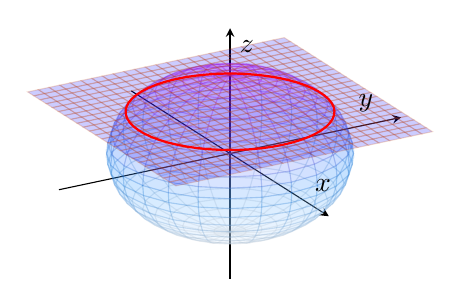
\begin{tikzpicture}
  \begin{axis}[
    view={60}{30},
    axis lines=center,
    xlabel={$x$}, ylabel={$y$}, zlabel={$z$},
    xmin=-2, xmax=2, ymin=-2, ymax=2, zmin=-2, zmax=2,
    ticks=none,
    enlargelimits=0.1
  ]
    % Draw Sphere outline
    \addplot3[surf, opacity=0.15, colormap/cool, domain=0:360, domain y=-90:90]
      ({1.5*cos(y)*cos(x)}, {1.5*cos(y)*sin(x)}, {1.5*sin(y)});
    
    % Intersecting plane z = k
    \addplot3[surf, color=blue, opacity=0.2, domain=-1.8:1.8, domain y=-1.8:1.8]
      (x, y, 0.8);
      
    % Circle Trace
    \addplot3[domain=0:360, samples=60, samples y=0, thick, color=red]
      ({sqrt(1.5^2 - 0.8^2)*cos(x)}, {sqrt(1.5^2 - 0.8^2)*sin(x)}, {0.8});
  \end{axis}
\end{tikzpicture}
\end{center}
\end{example}

\begin{example}
Find the trace of the plane $\mathcal{P} = \{(x, y, z) \mid -2x + 6y - 5z = 4\}$ with the plane $x = -1$:
\begin{align*}
-2(-1) + 6y - 5z &= 4 \\
2 + 6y - 5z &= 4 \\
6y - 5z &= 2 \implies z = \frac{6}{5}y - \frac{2}{5}
\end{align*}
The trace is a straight line in the plane $x = -1$.
\end{example}


\section{Quadric Surfaces}

A general \textbf{quadric surface} in $\mathbb{R}^3$ is given by the second-degree equation:
\[
Ax^2 + By^2 + Cz^2 + Dxy + Eyz + Fzx + ax + by + cz + d = 0
\]
When $D = E = F = 0$, the surface is in \textbf{standard position} (axes aligned with coordinate axes).

\begin{example}
The surface $x^2 + z^2 = 1$ is a circular cylinder aligned along the $y$-axis with radius $1$.
\begin{itemize}
    \item $z = 0$ trace: $x^2 = 1 \implies x = \pm 1$ (parallel lines along $y$).
    \item $x = 0$ trace: $z^2 = 1 \implies z = \pm 1$ (parallel lines along $y$).
\end{itemize}

\begin{center}
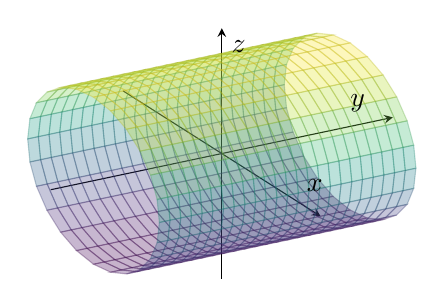
\begin{tikzpicture}
  \begin{axis}[
    view={60}{30},
    axis lines=center,
    xlabel={$x$}, ylabel={$y$}, zlabel={$z$},
    ticks=none,
    xmin=-1.5, xmax=1.5, ymin=-2, ymax=2, zmin=-1.5, zmax=1.5
  ]
    \addplot3[surf, opacity=0.3, colormap/viridis, domain=0:360, domain y=-1.5:1.5]
      ({cos(x)}, {y}, {sin(x)});
  \end{axis}
\end{tikzpicture}
\end{center}
\end{example}

\begin{example}
Consider the surface given by $x^2 + 4y^2 - z^2 = -1$.

\textbf{Traces:}
\begin{itemize}
    \item \textbf{$x = 0$ trace:} $4y^2 - z^2 = -1 \implies z = \pm\sqrt{4y^2 + 1}$. As $|y| \to \infty$, $z \approx \pm 2y$ (Hyperbola).
    \item \textbf{$y = 0$ trace:} $x^2 - z^2 = -1 \implies z = \pm\sqrt{x^2 + 1}$. As $|x| \to \infty$, $z \approx \pm x$ (Hyperbola).
    \item \textbf{$z = k$ trace:} $x^2 + 4y^2 = k^2 - 1$:
    \begin{itemize}
        \item $|k| = 1$: Single point at $(0, 0, \pm 1)$.
        \item $|k| < 1$: No trace (empty set).
        \item $|k| > 1$: Ellipse given by $x^2 + 4y^2 = k^2 - 1$.
    \end{itemize}
\end{itemize}

\begin{center}
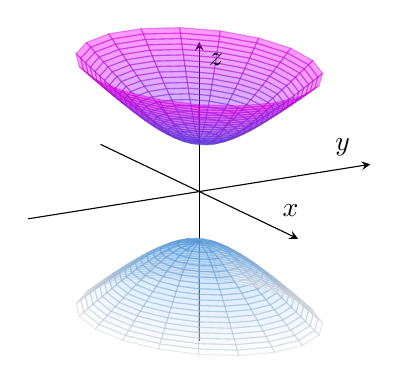
\begin{tikzpicture}
  \begin{axis}[
    view={60}{20},
    axis lines=center,
    xlabel={$x$}, ylabel={$y$}, zlabel={$z$},
    ticks=none,
    xmin=-3, xmax=3, ymin=-2, ymax=2, zmin=-3, zmax=3
  ]
    % Upper sheet: domain = z values [1, 2.5], domain y = angle [0, 360]
    \addplot3[surf, opacity=0.4, colormap/cool, domain=1:2.5, domain y=0:360, samples=20, samples y=20]
      ({sqrt(x^2-1)*cos(y)}, {0.5*sqrt(x^2-1)*sin(y)}, {x});
    % Lower sheet: domain = z values [-2.5, -1], domain y = angle [0, 360]
    \addplot3[surf, opacity=0.4, colormap/cool, domain=-2.5:-1, domain y=0:360, samples=20, samples y=20]
      ({sqrt(x^2-1)*cos(y)}, {0.5*sqrt(x^2-1)*sin(y)}, {x});
  \end{axis}
\end{tikzpicture}
\end{center}

\textbf{Why do cross-sectional ellipses fall on the surface?} \\
For any fixed height $z = k$ with $|k| > 1$, substituting $z = k$ fixes the value $k^2 - 1 > 0$ on the right side of $x^2 + 4y^2 = k^2 - 1$. This traces a locus of points $(x,y,k)$ whose horizontal distance components continuously satisfy the surface equation for that slice.
\end{example}

\end{document}